\part*{Annexes}
\sectionmark{Annexes}
\appendix
\let\oldaddtocontents\addtocontents
\def\addtocontents#1{%
   \def\tmpa{#1}%
   \def\tmpb{toc}%
   \ifx\tmpa\tmpb
      \def\tmpa{toca}%
   \fi
   \expandafter\oldaddtocontents\expandafter{\tmpa}}
\tableofcontentsA

\chapter{Liste des publications, conférences et associés}
\label{Ann:Communication}
\section{Publications}

\begin{itemize}
    \item J. Arnoux, A. Bonifati, A. Calteau, S. Dumbrava and G. Gautreau, "Integrating Complex Pangenome Graphs," 2024 IEEE 40th International Conference on Data Engineering Workshops (ICDEW), Utrecht, Netherlands, 2024, pp. 350-354, doi: 10.1109/ICDEW61823.2024.00052.
    \item J. Arnoux, J. Mainguy, L. Bry, Q. Fernandez de Grado, D. Vallenet, A. Calteau, "Panorama: A robust pangenome-based method for predicting and comparing biological systems across species"
\end{itemize}

\section{Présentation orale en conférence}

\begin{table}[htbp]
    \centering
    \begin{tabular}{l p{0.45\textwidth} p{0.28\textwidth}}
$\bullet$ Mai 2024 & Integrating Complex Pangenome Graphs,
& IEEE 40th International Conference on Data Engineering Workshops (ICDEW) à Utrecht, Pays-Bas \\
$\bullet$ Mai 2024 & PANORAMA: comparative pangenomics tools to explore interspecies diversity of microbial genomes & Journée de l'école doctorale SDSV \\
$\bullet$ Octobre 2023 & PANORAMA: comparative pangenomics tools to explore interspecies diversity of microbial genomes & The local pangenome à Alicante, Espagne \\
$\bullet$ Septembre 2023 & From Genomics to Pangenomics: the path to pangenome graph & The 20th MicroScope anniversary à Évry-Courcouronnes, France \\
$\bullet$ Juillet 2023 & PANORAMA: comparative pangenomics tools to explore interspecies diversity of microbial genomes & ISMB/ECCB à Lyon, France \\
$\bullet$ Juin 2023 & PANORAMA: comparative pangenomics tools to explore interspecies diversity of microbial genomes & Mini Congrès du Genoscope à Évry-Courcouronnes, France \\
$\bullet$ Juin 2022 & PANORAMA: comparative pangenomics tools to explore interspecies diversity of microbial genomes & Mini Congrès du Genoscope à Évry-Courcouronnes, France \\
    \end{tabular}
\end{table}

\newpage

\section{Posters et associés}

\begin{table}[htbp]
    \centering
    \begin{tabular}{l p{0.45\textwidth} p{0.28\textwidth}}
$\bullet$ Juillet 2023 :& PANORAMA: comparative pangenomics tools to explore interspecies diversity of microbial genomes & ISMB/ECCB à Lyon, France\\
$\bullet$ Mai 2023 :& PANORAMA: comparative pangenomics tools to explore interspecies diversity of microbial genomes & Journée de l'école doctorale SDSV \\
$\bullet$ Juillet 2022 :& PANORAMA: comparative pangenomics tools to explore interspecies diversity of microbial genomes & JOBIM à Rennes, France \\
$\bullet$ Juin 2022 :& PANORAMA: comparative pangenomics tools to explore interspecies diversity of microbial genomes & FEMS Conference on Microbiology à Belgrade, Serbie
\\
$\bullet$ Mai 2022 & PANORAMA: comparative pangenomics tools to explore interspecies diversity of microbial genomes & Doctoral school day SDSV \\
    \end{tabular}
\end{table}

\section{Certificats, Prix ET Bourses}

\begin{itemize}
    \item 2023 : Prix "science ouverte du logiciel libre de la recherche", "espoir" de la catégorie 'Scientifique et technique'
    \item 2022 : GDR BIM Bourse de voyage pour la conférence ISMB/ECCB, Lyon
    \item 2022 : 3\ieme{} place du D4GEN Hackathon
\end{itemize}


\chapter{Poster}

\section{FEMS Conference on Microbiology à  Belgrade, Serbie, 2022}

\begin{figure}[htbp]
    \centering
    \includegraphics[height=.55\textheight,angle=-90]{Annexes/PosterPANORAMAFEMS2022.jpg}
    \label{Ann:poster_fems}
\end{figure}

\newpage
\section{JOBIM  Journées Ouvertes en Biologie, Informatique et Mathématiques à Rennes, France, 2022}

\begin{figure}[htbp]
    \centering
    \includegraphics[width=.75\textwidth]{Annexes/PosterPANORAMA_JOBIM2022-1.jpg}
    \label{Ann:poster_jobim}
\end{figure}

\section{ISMB/ECCB à Lyon, France}

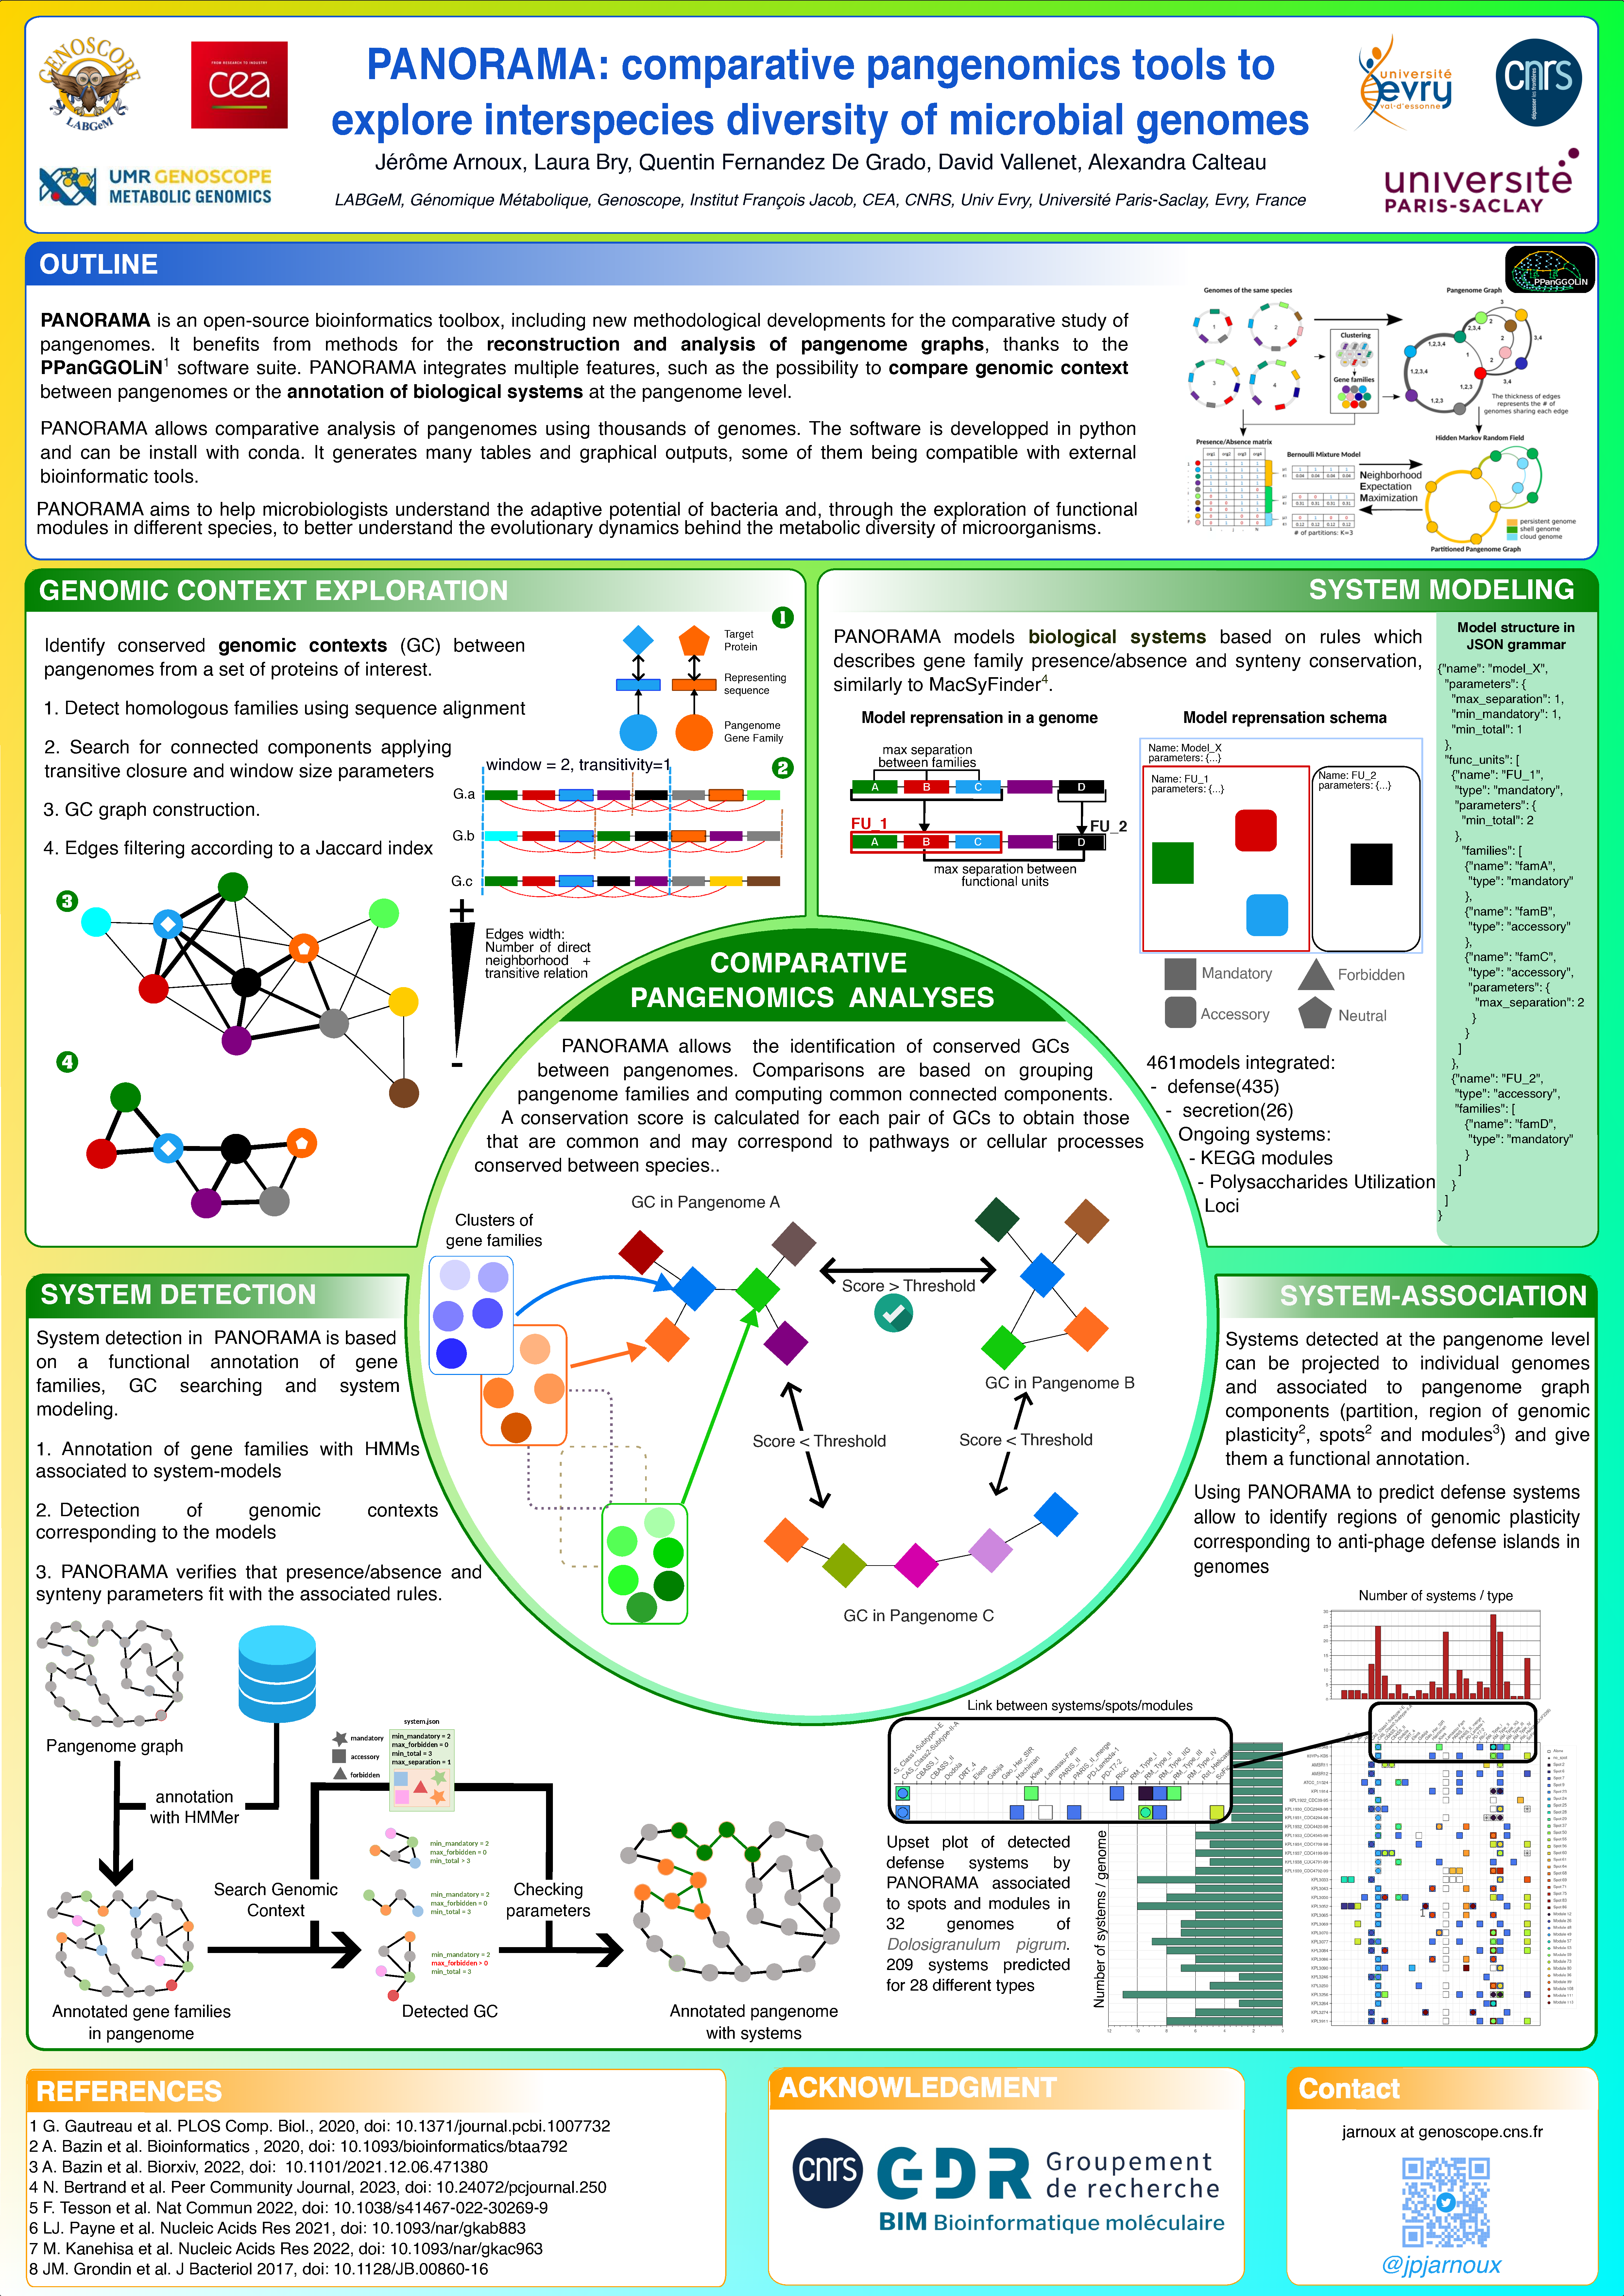
\includepdf[]{Annexes/POSTER.pdf}